\documentclass[11pt,a4paper]{article}

\usepackage[T1]{fontenc}
\usepackage[utf8]{inputenc}
\usepackage{lmodern}
\usepackage[magyar]{babel}
\usepackage{amsmath,amssymb}
\usepackage{newunicodechar}
\newunicodechar{ő}{\H{o}}
\newunicodechar{ű}{\H{u}}
\newunicodechar{Ő}{\H{O}}
\newunicodechar{Ű}{\H{U}}
\usepackage{geometry}
\geometry{margin=2.2cm}
\usepackage{longtable}
\usepackage{booktabs}
\usepackage{array}
\usepackage{tikz}
\usetikzlibrary{arrows.meta,positioning,calc}
\usepackage{hyperref}
\hypersetup{colorlinks=true,linkcolor=blue!50!black,urlcolor=blue!50!black}
\usepackage{enumitem}
\usepackage{xcolor}

\newcommand{\lean}[1]{\texttt{\small #1}}
% engedjük tördelni a hosszú elérési utakat és neveket a táblázatokban
\newcommand{\bk}{\allowbreak}
\newcommand{\pr}[1]{\href{https://github.com/leanprover-community/mathlib4/pull/#1}{\##1}}
\newcommand{\OK}{\textcolor{green!45!black}{\textbf{merge-elve}}}
\newcommand{\EL}{\textcolor{blue!55!black}{\textbf{még aktuális}}}
\newcommand{\OB}{\textcolor{gray}{\textbf{elavult}}}

\title{\textbf{A csatolt archívum Mathlib-hozzájárulásainak áttekintése}\\[2mm]
\large Mi van benne, mi került már be a mai Mathlibbe, és melyik
tematika\-elem kreditelismeréséhez használható}
\author{}
\date{Állapotfelmérés: Mathlib \lean{master} \lean{b87b4e892} (2026.\ augusztus 30.),
toolchain \lean{v4.\bk 34.\bk 0-rc1} vonal}

\begin{document}
\maketitle

\begin{abstract}
Az \lean{e525434d-\dots-aristotle(6).\bk tar.\bk gz} archívum kilenc önálló Mathlib-módosítási
javaslatot tartalmaz (tizenegy \lean{.\bk patch} fájlban, mert két javaslatnak több
verziója is el van téve), nyolc gépi ellenőrző Lean-fájlt és két újrahasznosítható
Python-eszközt. Ez a dokumentum (i) tételesen felsorolja, mi van az archívumban;
(ii) mindegyik javaslatról megmondja, hogy \emph{ma}, a nyilvános Mathlib
\lean{master} ágán (2026.\ augusztus 30.) még aktuális-e vagy már bekerült;
(iii) megadja a szerző eddigi \emph{összes} Mathlib PR-ját merge-státusszal
(köztük a már merge-elt Darboux-PR-t, amely \emph{nincs} benne ebben az
archívumban); és (iv) minden tételt hozzárendel a Kalkulus~I tantárgytematika
azon pontjához, amelynek kreditelismeréséhez felhasználható.
\end{abstract}

\tableofcontents

\section{Módszertan --- mit ellenőriztem ténylegesen}

Két, egymástól független ellenőrzés készült:

\begin{enumerate}[nosep]
  \item \textbf{Forráskód-szintű}: a nyilvános Mathlib-tárolóból lehúztam a
    \lean{master} ág mai fejét (\lean{b87b4e892}, 2026-08-30), és az archívum
    minden patch fájljára lefuttattam a \lean{git apply -{}-check} próbát,
    valamint kézzel megnéztem az érintett deklarációk mai állapotát.
    Egy patch, amely tisztán illeszkedik, biztosan \emph{nem} került még be;
    egy patch, amely azért nem illeszkedik, mert a javított hiba már nincs ott,
    bekerült.
  \item \textbf{PR-szintű}: a GitHub API-n keresztül lekérdeztem a szerző
    (\lean{attilavjda}) összes Mathlib-PR-ját és azok állapotát, valamint
    rákerestem, van-e más nyitott PR ugyanarra a helyre (ütközésveszély).
\end{enumerate}

\noindent
Amit \emph{nem} végeztem el ebben a menetben: teljes \lean{lake build Mathlib}
a mai masteren a patch-ekkel (ezt a korábbi menetek egy augusztus közepi
master-commiten futtatták le sikeresen). A ,,tisztán illeszkedik'' tehát
szövegszintű állítás; beküldés előtt a szokásos CI-futtatás pótolja a
fordítási ellenőrzést.

\section{Mi van az archívumban}

\begin{center}
\small
\begin{tabular}{@{}p{5.3cm}p{4.2cm}p{6.2cm}@{}}
\toprule
\textbf{Könyvtár} & \textbf{Tartalom} & \textbf{Megjegyzés}\\
\midrule
\lean{contribution/\bk *.\bk patch} & 11 patch fájl, 9 javaslat & két javaslatnak több verziója is benne van\\
\lean{RequestProject/\bk *.\bk lean} & 8 ellenőrző Lean-fájl & mindegyik \emph{módosítatlan} Mathlib ellen fordul, és \lean{rfl}/\lean{run\_\bk cmd} szinten hitelesíti a patch állítását\\
\lean{scripts/\bk } & \lean{deletion\_\bk scout.\bk py}, \lean{to\_\bk additive\_\bk twins.\bk py} & a duplikátum- és ,,kézzel írt \lean{to\_\bk additive} iker''-kereső eszközök\\
\lean{contribution/\bk scans/\bk } & \lean{dupscan} kimenetek & a jelöltlisták, amelyekből a javaslatok jöttek\\
\lean{pww-mapping/\bk } & ,,Proofs Without Words'' megfeleltetés & nem Mathlib-hozzájárulás\\
\bottomrule
\end{tabular}
\end{center}

\medskip
\noindent\textbf{Fontos: a Darboux-PR nincs ebben az archívumban.} A már
merge-elt \pr{42810} (\emph{fix(Analysis): two lemmas are copies of the one
above them}) sem patch, sem ellenőrző fájl formájában nem szerepel benne ---
az egy másik menet terméke. Ettől függetlenül a \S\ref{sec:prlista}
táblázatban szerepeltetem, mert a kreditelismerés szempontjából ez az egyik
legerősebb tétel.

\section{Az archívum kilenc javaslata és mai státuszuk}

\begingroup
\small
\begin{longtable}{@{}>{\raggedright\arraybackslash}p{0.45cm}>{\raggedright\arraybackslash}p{4.4cm}>{\raggedright\arraybackslash}p{4.2cm}>{\raggedright\arraybackslash}p{5.2cm}@{}}
\toprule
\textbf{\#} & \textbf{Javaslat} & \textbf{Érintett Mathlib-fájl(ok)} & \textbf{Státusz ma (master \lean{b87b4e892})}\\
\midrule
\endfirsthead
\toprule
\textbf{\#} & \textbf{Javaslat} & \textbf{Érintett Mathlib-fájl(ok)} & \textbf{Státusz ma}\\
\midrule
\endhead
\bottomrule
\endfoot
1 & \lean{@[to\_\bk additive]} a \lean{prod\_\bk Ico\_\bk reflect} / \lean{prod\_\bk range\_\bk reflect} lemmákra, a kézzel írt additív ikrek törlése
  & \lean{Algebra/\bk BigOperators/\bk Intervals.\bk lean}, \lean{.\bk .\bk .\bk /\bk NatAntidiagonal.\bk lean}
  & \OK{} --- \pr{42592} (2026-08-10) és \pr{42763} (2026-08-15). A mai fájlban ott a \lean{@[to\_\bk additive]}, az ikrek eltűntek; a patch már nem illeszkedik.\\
\addlinespace
2 & \lean{NatAntidiagonal.\bk lean}: a holtponttá vált \lean{N}, \lean{[AddCommMonoid N]} szekcióváltozók törlése
  & \lean{Algebra/\bk BigOperators/\bk NatAntidiagonal.\bk lean}
  & \OK{} --- \pr{42907} (2026-08-18). A mai sor: \lean{variable \{M : Type*\} [CommMonoid M]}.\\
\addlinespace
3 & Fordított háromszög-egyenlőtlenség deduplikálása ($\bigl||a|-|b|\bigr|\le|a-b|$ kétszer van bizonyítva)
  & \lean{Algebra/\bk Order/\bk Group/\bk Unbundled/\bk Abs.\bk lean} (130.\ sor), \lean{Algebra/\bk Order/\bk Group/\bk Abs.\bk lean} (119.\ sor), \lean{Analysis/\bk Normed/\bk Order/\bk Lattice.\bk lean}
  & \EL{} --- mindkét példány megvan a masteren, a patch \emph{tisztán illeszkedik}. Más nyitott PR nem érinti. Beküldésre kész.\\
\addlinespace
4 & \lean{SameRay}: a felesleges \lean{[IsStrictOrderedRing R]} és a \lean{@[nolint unusedArguments]} törlése (a fájlbeli TODO teljesítése) --- 61 lemma veszít el egy feltételt
  & \lean{LinearAlgebra/\bk Ray.\bk lean}, \lean{Analysis/\bk Convex/\bk Side.\bk lean}
  & \EL{} --- a TODO, a \lean{nolint} és a feltétel ma is ott van; a patch \emph{tisztán illeszkedik}. Ez a legnagyobb matematikai hozadékú tétel a maradékból.\\
\addlinespace
5 & \lean{Finset.\bk range\_\bk add} vs.\ \lean{Finset.\bk range\_\bk add\_\bk eq\_\bk union}: két különböző fájlban, két bizonyítással, ugyanaz az állítás
  & \lean{Algebra/\bk Group/\bk Nat/\bk Range.\bk lean} (34.\ sor), \lean{Order/\bk Interval/\bk Finset/\bk Nat.\bk lean} (233.\ sor), \lean{Combinatorics/\bk Additive/\bk AP/\bk Three/\bk Defs.\bk lean}
  & \EL{} --- mindkettő megvan, a patch \emph{tisztán illeszkedik}.\\
\addlinespace
6 & A skatulyaelv modul-docstringjének javítása (Lean~3-as modulnevek, nem létező deklarációnevek)
  & \lean{Combinatorics/\bk Pigeonhole.\bk lean}
  & \EL{} --- a docstring ma is a régi neveket sorolja (pl.\ \lean{Set.\bk infinite.\bk exists\_\bk ne\_\bk map\_\bk eq\_\bk of\_\bk mapsTo}); a patch \emph{tisztán illeszkedik}.\\
\addlinespace
7 & Elavult docstring-hivatkozások javítása 6 fájlban (\lean{factorization\_\bk choose\_\bk le}, \lean{interval\bk Gaps\bk Within\_\bk injective}, \lean{div\_\bk le\_\bk div\_\bk iff}/\lean{Linear\bk Ordered\bk Semifield}, \lean{*.\bk locallyFiniteOrder}, Lean~3 modulnevek)
  & \lean{Data/\bk Nat/\bk Choose/\bk Factorization.\bk lean}, \lean{Data/\bk Nat/\bk Choose/\bk Basic.\bk lean}, \lean{Order/\bk Interval/\bk Finset/\bk \{Gaps,\bk Defs,\bk Basic\}}, \lean{Algebra/\bk Order/\bk Group/\bk Unbundled/\bk Basic.\bk lean}
  & \EL{} --- mind a hat hely változatlan; a patch \emph{tisztán illeszkedik}.\\
\addlinespace
8 & Három ,,elavult átnevezési TODO'' teljesítése: \lean{Multiset.\bk map\_\bk filter'}, Schwarz-lemma \lean{\dots\_\bk dslope\_\bk eq\_\bk div'}, \lean{IsLocalization.\bk surj''}
  & \lean{Data/\bk Multiset/\bk Filter.\bk lean}, \lean{Analysis/\bk Complex/\bk Schwarz.\bk lean}, \lean{RingTheory/\bk Localization/\bk InvSubmonoid.\bk lean}, \lean{AlgebraicGeometry/\bk AffineScheme.\bk lean}
  & \textbf{részben lekörözve}: a \lean{Multiset} rész \OK{} (\pr{42970}, más szerző, 2026-08-25); a \lean{surj''} részre \emph{van} nyitott, idegen PR (\pr{42967}); a Schwarz-rész \EL{} és szabad. Frissített patch mellékelve.\\
\addlinespace
9 & \lean{Nat.\bk not\_\bk two\_\bk dvd\_\bk bit1} vs.\ \lean{Nat.\bk two\_\bk not\_\bk dvd\_\bk two\_\bk mul\_\bk add\_\bk one} (azonos állítás, azonos bizonyítás, Lean~3-as ,,\lean{bit1}'' név)
  & \lean{Data/\bk Nat/\bk Init.\bk lean} (373.\ sor), \lean{Algebra/\bk Group/\bk Nat/\bk Even.\bk lean} (53.\ sor), \lean{Data/\bk Nat/\bk Squarefree.\bk lean}
  & \EL{} --- a duplikáció ma is fennáll. \textbf{Figyelem}: az archívumban csak az ellenőrző Lean-fájl van benne, a hivatkozott \lean{nat-not-two-dvd-bit1-dedup.\bk patch} \emph{hiányzik}, azt újra kell gyártani.\\
\end{longtable}
\endgroup

\medskip
\noindent
Összefoglalva: a kilencből \textbf{kettő már bent van} a Mathlibben (1., 2.),
\textbf{öt teljesen szabad és beküldésre kész} (3., 4., 5., 6., 7.),
\textbf{egy részben lekörözték} (8.), \textbf{egynél a patch fájl hiányzik}
de a hiba még javítható (9.).

\begin{center}
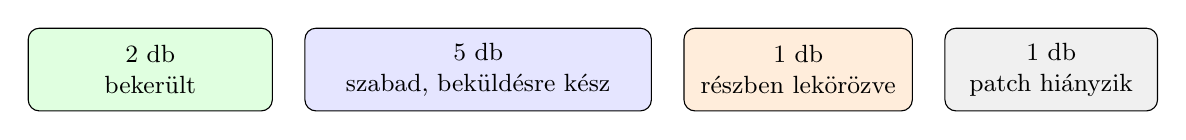
\begin{tikzpicture}[font=\small,node distance=4mm]
  \node[draw,rounded corners,fill=green!12,minimum width=3.1cm,minimum height=1.05cm,align=center] (a) {2 db\\bekerült};
  \node[draw,rounded corners,fill=blue!10,minimum width=4.4cm,minimum height=1.05cm,align=center,right=of a] (b) {5 db\\szabad, beküldésre kész};
  \node[draw,rounded corners,fill=orange!14,minimum width=2.9cm,minimum height=1.05cm,align=center,right=of b] (c) {1 db\\részben lekörözve};
  \node[draw,rounded corners,fill=gray!12,minimum width=2.7cm,minimum height=1.05cm,align=center,right=of c] (d) {1 db\\patch hiányzik};
\end{tikzpicture}
\end{center}

\section{A szerző összes Mathlib-PR-ja és merge-státusza}
\label{sec:prlista}

A lenti lista a GitHubról származik (2026-08-30-i lekérdezés,
\lean{author:attilavjda}); a merge-eltek megtalálhatók a \lean{master}
történetében is, ezért az ellenőrzés kétszeres.

\subsection{Merge-elt PR-ok (6~db)}

\begingroup
\small
\begin{longtable}{@{}>{\raggedright\arraybackslash}p{1.3cm}>{\raggedright\arraybackslash}p{1.6cm}>{\raggedright\arraybackslash}p{6.3cm}>{\raggedright\arraybackslash}p{5.2cm}@{}}
\toprule
\textbf{PR} & \textbf{Merge} & \textbf{Cím} & \textbf{Tartalom / kapcsolat}\\
\midrule
\endfirsthead
\bottomrule
\endfoot
\pr{42493} & 2026-08-10 & \lean{chore(GroupTheory/\bk Complement)}: deduplicate \lean{IsComplement.\bk card\_\bk mul} & algebrai duplikáció; nincs az archívumban\\
\addlinespace
\pr{42592} & 2026-08-10 & \lean{chore(Algebra/\bk BigOperators)}: generate \lean{sum\_\bk Ico\_\bk reflect}/\lean{sum\_\bk range\_\bk reflect} with \lean{to\_\bk additive} & \textbf{az archívum 1.\ javaslata}\\
\addlinespace
\pr{42579} & 2026-08-13 & \lean{fix(Analysis/\bk Convex/\bk Basic)}: \lean{Monotone.\bk convex\_\bk lt}/\lean{convex\_\bk gt} state the wrong set & \emph{tartalmi hibajavítás} konvexitásban; nincs az archívumban\\
\addlinespace
\pr{42763} & 2026-08-15 & \lean{chore(Algebra/\bk BigOperators)}: add \lean{to\_\bk additive} for expectation and antidiagonal lemmas & \textbf{az 1.\ javaslat antidiagonál-fele} + várható érték\\
\addlinespace
\pr{42810} & 2026-08-18 & \lean{fix(Analysis)}: two lemmas are copies of the one above them & \textbf{a Darboux-PR}: \lean{Analysis/\bk Calculus/\bk Darboux.\bk lean} \lean{\dots\_\bk of\_\bk le\_\bk of\_\bk ge} (a saját docstringjének ellentmondó másolat) és \lean{UpperHalfPlane/\bk Metric.\bk lean} \lean{le\_\bk dist\_\bk iff\_\bk le\_\bk dist\_\bk coe\_\bk center}; nincs az archívumban\\
\addlinespace
\pr{42907} & 2026-08-18 & \lean{chore(\dots/\bk NatAntidiagonal)}: remove unused variable & \textbf{az archívum 2.\ javaslata}\\
\end{longtable}
\endgroup

\subsection{Nyitott PR-ok (9~db, 2026-08-30-i állapot)}

Ezek egyike sem szerepel az archívumban, de a kreditdossziéban érdemes
felsorolni őket (,,folyamatban''):

\begingroup
\small
\begin{longtable}{@{}>{\raggedright\arraybackslash}p{1.3cm}>{\raggedright\arraybackslash}p{8.9cm}>{\raggedright\arraybackslash}p{4.2cm}@{}}
\toprule
\textbf{PR} & \textbf{Cím} & \textbf{Témakör}\\
\midrule
\endfirsthead
\bottomrule
\endfoot
\pr{42082} & \lean{feat(FieldTheory)}: reduce Frobenius powers modulo the extension degree & testelmélet (új tartalom)\\
\pr{42339} & \lean{feat}: add diagonal \lean{iSup} and \lean{iInf} lemmas & rendezéselmélet, szuprémum\\
\pr{42499} & \lean{doc(Data/\bk ENat,ENNReal)}: fix swapped docstring on \lean{mul\_\bk iInf\_\bk of\_\bk ne} & dokumentáció\\
\pr{42505} & \lean{chore(Algebra/\bk Tropical/\bk Basic)}: deduplicate five pairs of lemmas & deduplikáció\\
\pr{42509} & \lean{chore(Analysis/\bk Normed/\bk Lp/\bk PiLp)}: fix stale docstring cross-references & dokumentáció\\
\pr{42533} & \lean{chore(\dots/\bk Pow/\bk Real)}: deprecate six misnamed duplicate log/rpow lemmas & elemi függvények, deduplikáció\\
\pr{42583} & \lean{chore(Analysis/\bk Calculus/\bk FDeriv/\bk Prod)}: deprecate \lean{differentiable*\_\bk finCons'} duplicates & derivált\\
\pr{42764} & \lean{chore(GroupTheory)}: make \lean{smul\_\bk eq\_\bk self\_\bk of\_\bk mem\_\bk zpowers} \lean{to\_\bk additive} & \lean{to\_\bk additive}\\
\pr{42823} & \lean{chore}: let \lean{to\_\bk additive} generate hand-written additive twins & az archívumbeli eszköz terméke\\
\end{longtable}
\endgroup

\noindent
Két korábbi PR lezárult merge nélkül (\pr{41973}, \pr{42399} --- a diagonális
\lean{iSup} téma, amelyet a \pr{42339} vitt tovább), egy pedig
összevonás miatt (\pr{42746} $\to$ \pr{42763}).

\section{Kreditelismerés: melyik tétel melyik tematikaelemet fedi}

A tematikai pontok nevei a Kalkulus~I ,,Tantárgy tartalma'' listájából valók,
ugyanabban a bontásban, ahogy a \lean{kalkulus\_\bk kategoriaelmelet.\bk pdf}
megfeleltetési táblázata használja. A ,,kapcsolat erőssége'' azt jelzi,
mennyire közvetlen az összefüggés a tematikaelemmel: \textbf{erős} = a lemma
maga a tananyag állítása; \textbf{közepes} = a tananyag-állítás bizonyításához
használt Mathlib-infrastruktúra; \textbf{gyenge} = rokon terület.

\begingroup
\small
\begin{longtable}{@{}>{\raggedright\arraybackslash}p{4.5cm}>{\raggedright\arraybackslash}p{1.9cm}>{\raggedright\arraybackslash}p{4.2cm}>{\raggedright\arraybackslash}p{1.8cm}>{\raggedright\arraybackslash}p{2.2cm}@{}}
\toprule
\textbf{Tematikai pont} & \textbf{Gyakorlat} & \textbf{Mathlib-tétel} & \textbf{Erősség} & \textbf{Állapot}\\
\midrule
\endfirsthead
\toprule
\textbf{Tematikai pont} & \textbf{Gyakorlat} & \textbf{Mathlib-tétel} & \textbf{Erősség} & \textbf{Állapot}\\
\midrule
\endhead
\bottomrule
\endfoot
Nevezetes egyenlőtlenségek (háromszög-egyenlőtlenség, abszolút érték)
  & 1.11--1.13
  & 3.: fordított háromszög-egyenlőtlenség deduplikálása
  & erős
  & \EL{}\\
\addlinespace
Teljes indukció; véges összegek (Gauss-összeg, teleszkóp)
  & 1.14 a), 1.17
  & 1.: \lean{sum\_\bk range\_\bk reflect} (ezzel bizonyítja a Mathlib a Gauss-összeget)
  & erős
  & \OK{} \pr{42592}\\
\addlinespace
Teljes indukció; binomiális együtthatók
  & 1.19
  & 1.: \lean{sum\_\bk Ico\_\bk reflect} (a \lean{Nat.\bk sum\_\bk range\_\bk choose\_\bk halfway} bizonyításában), ill.\ 2.
  & erős
  & \OK{} \pr{42592}, \pr{42763}, \pr{42907}\\
\addlinespace
Véges összegek indexhalmazának felbontása
  & 1.14, 1.17
  & 5.: \lean{Finset.\bk range\_\bk add} deduplikálás
  & közepes
  & \EL{}\\
\addlinespace
A valós számtest; irracionalitás, paritásérvek
  & 1.9 ($\sqrt2\notin\mathbb Q$)
  & 9.: \lean{Nat.\bk not\_\bk two\_\bk dvd\_\bk bit1} deduplikálás
  & közepes
  & \EL{} (patch pótlandó)\\
\addlinespace
Skatulyaelv (Dirichlet), diofantikus approximáció
  & 1.10
  & 6.: \lean{Combinatorics/\bk Pigeonhole.\bk lean} docstring-javítás
  & közepes
  & \EL{}\\
\addlinespace
Felső/alsó határ, intervallumok, rendezett struktúrák
  & 1.3--1.5, 1.12
  & 7.: elavult docstring-hivatkozások (\lean{Order/\bk Interval/\bk Finset/\bk *}, \lean{Order/\bk Group/\bk Unbundled/\bk Basic})
  & gyenge
  & \EL{}\\
\addlinespace
Binomiális együtthatók, prímfelbontás
  & 1.19
  & 7.: \lean{Data/\bk Nat/\bk Choose/\bk *} docstring-javítás
  & közepes
  & \EL{}\\
\addlinespace
Konvexitás és a második derivált
  & 4.8/18, 4.13
  & \pr{42579}: \lean{Monotone.\bk convex\_\bk lt}/\lean{convex\_\bk gt} rossz halmazt állít --- \emph{tartalmi} hibajavítás
  & erős
  & \OK{}\\
\addlinespace
Konvexitás, félterek, konvex geometria
  & 4.13
  & 4.: \lean{SameRay} feltételtörlés + 61 lemma általánosítása (\lean{Analysis/\bk Convex/\bk Side.\bk lean})
  & közepes
  & \EL{}\\
\addlinespace
Monotonitás és derivált; a derivált Darboux-tulajdonsága
  & 4.8/18, 4.11
  & \pr{42810}: \lean{Analysis/\bk Calculus/\bk Darboux.\bk lean} duplikátum javítása
  & erős
  & \OK{}\\
\addlinespace
Differenciálhatóság, deriválási szabályok
  & 4.1--4.3
  & \pr{42583} (nyitott): \lean{FDeriv/\bk Prod} duplikátumok
  & közepes
  & nyitott\\
\addlinespace
Elemi függvények (logaritmus, hatvány)
  & 2.19--2.20, 3.7
  & \pr{42533} (nyitott): félrenevezett \lean{log}/\lean{rpow} duplikátumok
  & közepes
  & nyitott\\
\addlinespace
Szuprémum, teljességi axióma (univerzális tulajdonság)
  & 1.4, 1.5
  & \pr{42339} (nyitott): diagonális \lean{iSup}/\lean{iInf} lemmák
  & közepes
  & nyitott\\
\end{longtable}
\endgroup

\subsection{Javasolt kreditdosszié-szerkezet}

A kreditelismerési kérelemben érdemes háromszintűen érvelni:

\begin{enumerate}[nosep]
  \item \textbf{Bizonyítottan elfogadott hozzájárulás} (6 merge-elt PR).
    Ezek közül tantárgyilag a legerősebb kettő:
    \pr{42810} (Darboux-tétel környéke $\to$ ,,monotonitás és derivált'')
    és \pr{42579} (,,konvexitás és a második derivált'' --- ez nem kozmetika,
    hanem \emph{hibás állítás} javítása); a nagy összegzős hármas
    (\pr{42592}, \pr{42763}, \pr{42907}) a ,,teljes indukció, véges összegek,
    binomiális együtthatók'' blokkot fedi le.
  \item \textbf{Folyamatban lévő hozzájárulás} (9 nyitott PR) --- tematikánként
    a fenti táblázat szerint.
  \item \textbf{Elkészült, gépileg ellenőrzött, beküldésre kész munka}
    (az archívum 3.--7.\ javaslata + a 8.\ maradéka): ezekhez patch \emph{és}
    módosítatlan Mathlib ellen forduló Lean-ellenőrző fájl is tartozik, ami
    önmagában is bemutatható munkatermék.
\end{enumerate}

\section{Ütközések és teendők a maradék öt-hat javaslatnál}

\begin{itemize}[nosep]
  \item \textbf{3.\ (fordított háromszög-egyenlőtlenség).} Szabad, tisztán
    illeszkedik. Deprekációs ciklust igényel (két rövid név aliasként marad),
    ezért érdemes a dokumentumban is szereplő ,,konzervatív változatot''
    (a rövid név marad, a hosszút deprekáljuk) alternatívaként felajánlani a
    review-ban.
  \item \textbf{4.\ (\lean{SameRay}).} Szabad, és a fájlban lévő maintainer-TODO
    teljesítése, ami erős érv a reviewban. A diff nagy része a
    \lean{omit [IsStrictOrderedRing R] in} sorokból jön; a leírásban érdemes
    kiemelni, hogy a törlés maga 3 sor.
  \item \textbf{5.\ (\lean{Finset.\bk range\_\bk add}).} Szabad, apró; egyetlen
    hívási hely van a Mathlibben.
  \item \textbf{6.\ és 7.\ (docstringek).} Szabad, kockázatmentes, gyors
    review-jú tételek; a szerzőnek már van hasonló nyitott PR-ja (\pr{42509}),
    érdemes lehet ezeket egy PR-ba fésülni vagy a meglévőre hivatkozni.
  \item \textbf{8.\ (átnevezési TODO-k).} A három elemből a \lean{Multiset}-eset
    már nem aktuális (\pr{42970}), a \lean{IsLocalization.\bk surj''}-esetre pedig
    más nyitott PR-t adott be (\pr{42967}) --- ezt \emph{nem} érdemes párhuzamosan
    beküldeni. A Schwarz-lemma átnevezése szabad; a mellékelt
    \lean{patches/\bk stale-rename-todos-2026-08-30.\bk patch} pontosan ezt a
    csökkentett változatot tartalmazza (a \lean{Multiset}-rész nélkül).
  \item \textbf{9.\ (\lean{not\_\bk two\_\bk dvd\_\bk bit1}).} A duplikáció áll, de a patch
    fájl hiányzik az archívumból; a leírásból (átnevezés + deprekált alias +
    három hívási hely a \lean{Squarefree.\bk lean}-ben) egyszerűen újragyártható.
\end{itemize}

\section{Mellékelt fájlok}

A \lean{pr-attekintes/\bk patches/\bk } könyvtárban azok a patch-ek találhatók,
amelyek a mai masteren \emph{tisztán illeszkednek} (a \lean{git apply -{}-check}
ma lefutott mindegyikre):

\begin{center}
\footnotesize
\begin{tabular}{@{}ll@{}}
\toprule
\textbf{Fájl} & \textbf{Javaslat}\\
\midrule
\lean{abs-abs-sub-abs-dedup.\bk patch} & 3.\ fordított háromszög-egyenlőtlenség\\
\lean{sameray-drop-isstrictorderedring.\bk patch} & 4.\ \lean{SameRay}\\
\lean{finset-range-add-dedup.\bk patch} & 5.\ \lean{Finset.\bk range\_\bk add}\\
\lean{pigeonhole-docstring-fixes.\bk patch} & 6.\ skatulyaelv docstring\\
\lean{stale-docstring-references.\bk patch} & 7.\ elavult docstring-hivatkozások\\
\lean{stale-rename-todos-2026-08-30.\bk patch} & 8.\ maradéka (Schwarz + \lean{surj''}), mai masterre újragenerálva\\
\bottomrule
\end{tabular}
\end{center}

\noindent
Alkalmazás:
\lean{git -C <mathlib-checkout> apply pr-attekintes/\bk patches/\bk <fájl>}.

\end{document}
